\begin{abox}
	Exam Electronics-1
	\end{abox}
\begin{enumerate}
	\item In one of the following circuits, negative feedback does not operate for a negative input. Which one is it? The opamps are running from $\pm 15 \mathrm{~V}$ supplies.
{	\exyear{GATE 2010}}
\begin{tasks}(2)
\task[\textbf{A.}] \begin{figure}[H]
	\centering
	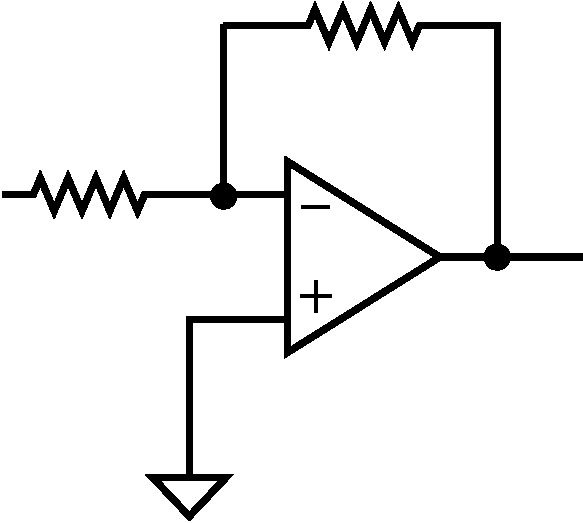
\includegraphics[height=3.5cm,width=4cm]{diagram-20210912(9)-crop}
\end{figure}
\task[\textbf{B.}] \begin{figure}[H]
	\centering
	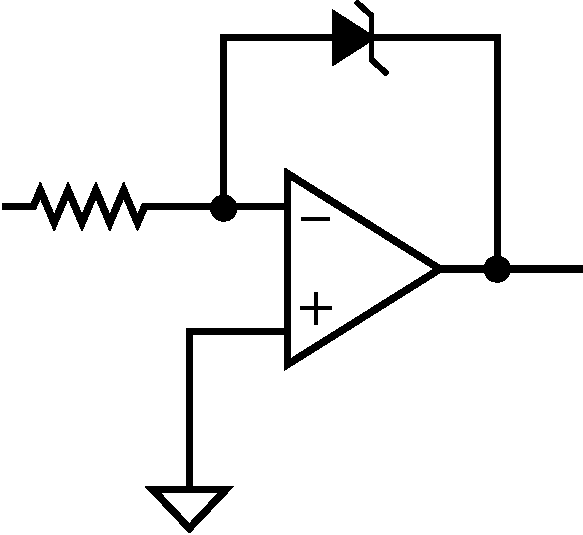
\includegraphics[height=3.5cm,width=4cm]{diagram-20210912(10)-crop}
\end{figure}
\task[\textbf{C.}] \begin{figure}[H]
	\centering
	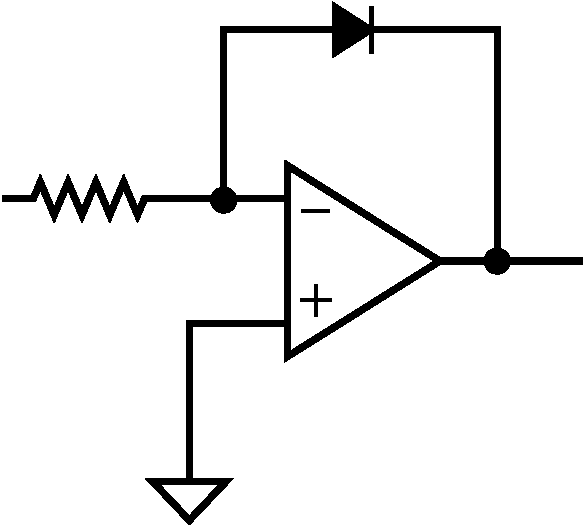
\includegraphics[height=3.5cm,width=4cm]{diagram-20210912(11)-crop}
\end{figure}
\task[\textbf{D.}] \begin{figure}[H]
	\centering
	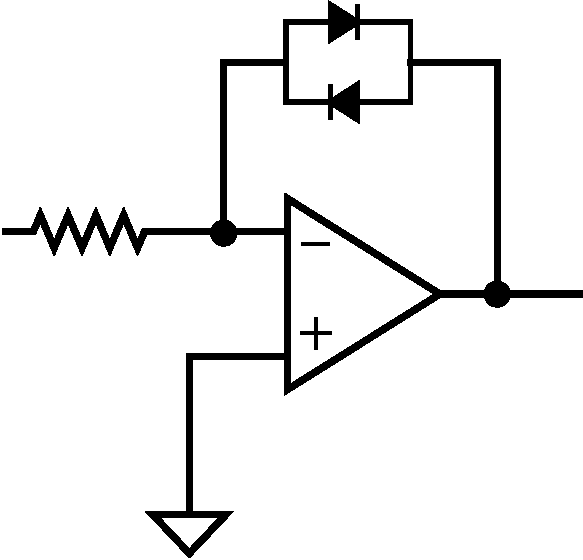
\includegraphics[height=3.5cm,width=4cm]{diagram-20210912(12)-crop}
\end{figure}
\end{tasks}
\begin{answer}
So the correct answer is \textbf{Option (C)}
\end{answer}
	\item Which of the following statements is CORRECT for a common emitter amplifier circuit?
	{\exyear{GATE 2011}}
\begin{tasks}(1)
\task[\textbf{A.}] The output is taken from the emitter
\task[\textbf{B.}] There is $180^{\circ}$ phase shift between input and output voltages
\task[\textbf{C.}] There is no phase shift between input and output voltages
\task[\textbf{D.}] Both $p-n$ junctions are forward biased
\end{tasks}
\begin{answer}
So the correct answer is \textbf{Option (B)}
\end{answer}
	\item If the peak output voltage of a full wave rectifier is $10 \mathrm{~V}$, its d.c. voltage is
{	\exyear{GATE 2012}}
\begin{tasks}(4)
\task[\textbf{A.}] $10.0 \mathrm{~V}$
\task[\textbf{B.}] $7.07 \mathrm{~V}$
\task[\textbf{C.}] $6.36 \mathrm{~V}$
\task[\textbf{D.}] $3.18 \mathrm{~V}$
\end{tasks}
\begin{answer}
\begin{align*}
V_{d c}&=\frac{2 V_{m}}{\pi}=\frac{2 \times 10}{22 / 7}\\&=\frac{14 \times 10}{22}=\frac{70}{11}=6.36 \mathrm{~V}
\end{align*}
So the correct answer is \textbf{Option (C)}
\end{answer}
	\item Consider the following circuit in which the current gain $\beta_{d c}$ of the transistor is 100 .\\
	\begin{figure}[H]
		\centering
		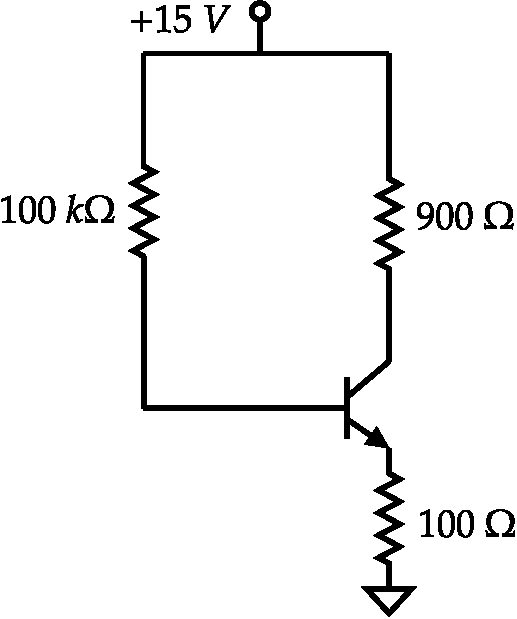
\includegraphics[height=6cm,width=5cm]{diagram-20210913(23)-crop}
	\end{figure}
	Which one of the following correctly represents the load line (collector current $\mathrm{I}_{\mathrm{C}}$ with respect to collector-emitter voltage $\mathrm{V}_{\mathrm{CE}}$ ) and Q-point of this circuit?
{	\exyear{GATE 2012}}
\begin{tasks}(2)
\task[\textbf{A.}]\begin{figure}[H]
	\centering
	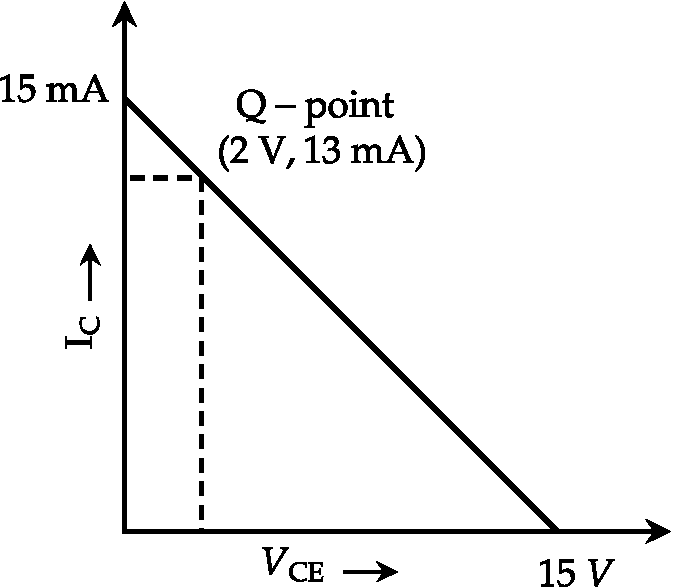
\includegraphics[height=4.5cm,width=5cm]{diagram-20210913(24)-crop}
\end{figure}
\task[\textbf{B.}] \begin{figure}[H]
	\centering
	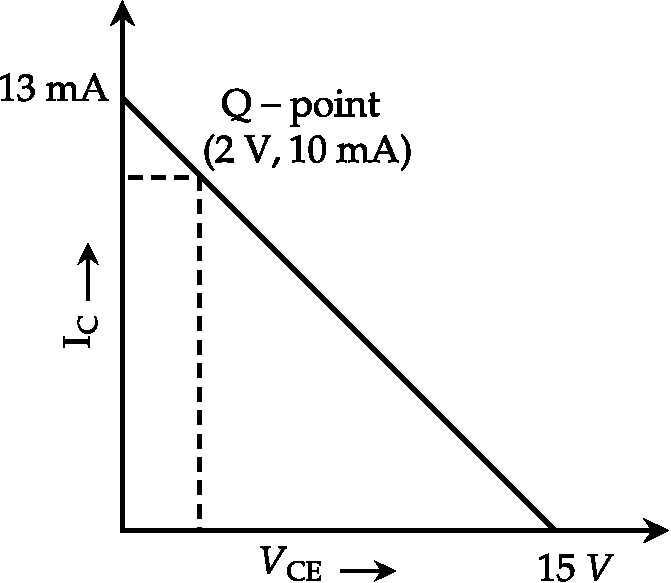
\includegraphics[height=4.5cm,width=5cm]{diagram-20210913(25)-crop}
\end{figure}
\task[\textbf{C.}] \begin{figure}[H]
	\centering
	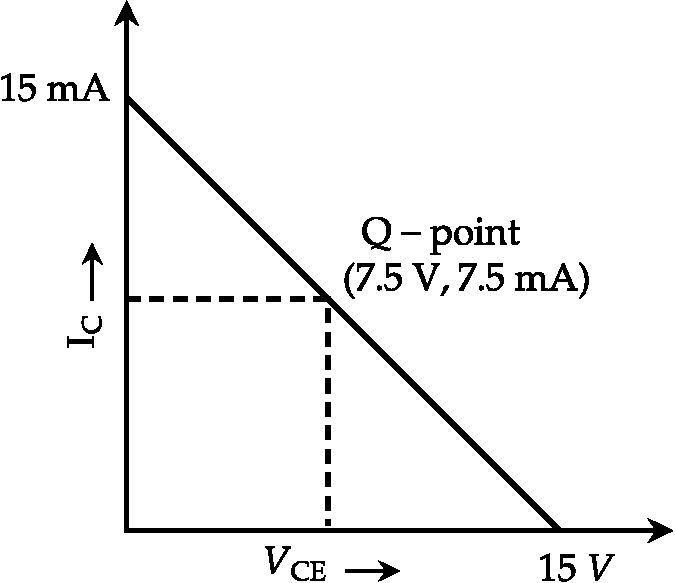
\includegraphics[height=4.5cm,width=5cm]{diagram-20210913(26)-crop}
\end{figure}
\task[\textbf{D.}] \begin{figure}[H]
	\centering
	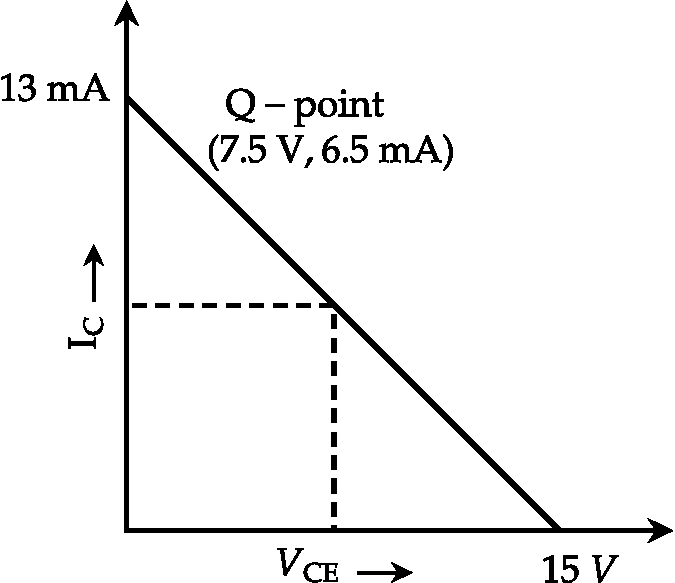
\includegraphics[height=4.5cm,width=5cm]{diagram-20210913(27)-crop}
\end{figure}
\end{tasks}
\begin{answer}
\begin{align*}
I_{B}&=\frac{V_{C C}-V_{B E}}{R_{B}+R_{E}}=\frac{15-0.7}{100 \times 10^{3}+100} \approx \frac{14.3}{100} m A\\
I_{C} \approx \beta I_{B} \approx 14.3 m A \approx 13 m A, V_{C E}&=V_{C C}-I_{C}\left(R_{C}+R_{E}\right)\\&=15-(900+100) \times 13 \times 10^{-3}=2 V\\
I_{C, S a t}&=\frac{\mathrm{V}_{\mathrm{CC}}}{\mathrm{R}_{\mathrm{C}}+R_{E}}=\frac{15}{1000}=15 \mathrm{~mA}
\end{align*}
So the correct answer is \textbf{Option (A)}
\end{answer}
	\item The current gain of the transistor in the following circuit is $\beta_{d c}=100$. The value of collector current $I_{C}$ is----------- $m A$
{	\exyear{GATE 2014}}
\begin{figure}[H]
\centering
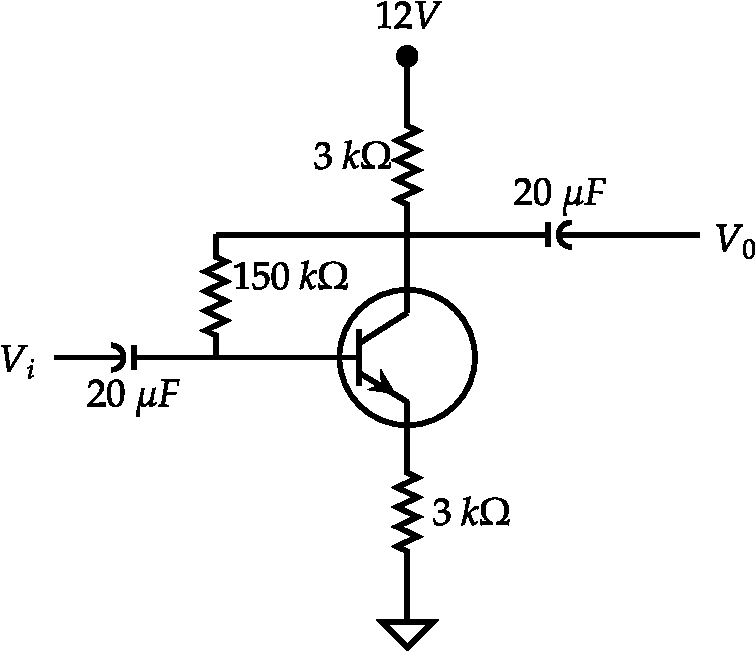
\includegraphics[height=7cm,width=8cm]{diagram-20210913(43)-crop}
\end{figure}
\begin{answer}
\begin{align*}
I_{B}&=\frac{V_{C C}-V_{B E}}{R_{B}+\beta\left(R_{C}+R_{E}\right)}=\frac{12-0}{150+100(3+3)}\\&=0.016 \mathrm{~mA} \Rightarrow I_{C}=\beta I_{B}=1.6 \mathrm{~mA}
\end{align*}
\end{answer}
	\item A low pass filter is formed by a resistance $R$ and a capacitance $C .$ At the cut-off angular frequency $\omega_{C}=\frac{1}{R C}$ the voltage gain and the phase of the output voltage relative to the input voltage respectively are
{	\exyear{GATE 2014}}
\begin{tasks}(4)
\task[\textbf{A.}] $0.71$ and $45^{\circ}$
\task[\textbf{B.}]  $0.71$ and $-45^{\circ}$
\task[\textbf{C.}] $0.5$ and $-90^{\circ}$
\task[\textbf{D.}] $0.5$ and $90^{\circ}$
\end{tasks}
\begin{answer}
\begin{align*}
\frac{v_{0}}{v_{i n}}&=\frac{X_{C}}{R+X_{C}}=\frac{1}{\frac{R}{X_{C}}+1}\\&=\frac{1}{1+j \omega C R}\\
At \omega&=\omega_{C}=\frac{1}{R C} \Rightarrow \frac{v_{0}}{v_{i n}}=\frac{1}{1+j}\\&=\frac{1}{\sqrt{2} e^{j 45^{0}}}=\frac{1}{\sqrt{2}} e^{-j 45^{0}}
\end{align*}
So the correct answer is \textbf{Option (B)}
\end{answer}
	\item A time varying signal $V_{i n}$ is fed to an op-amp circuit with output signal $V_{o}$ as shown in the figure below.\\
	\begin{figure}[H]
		\centering
		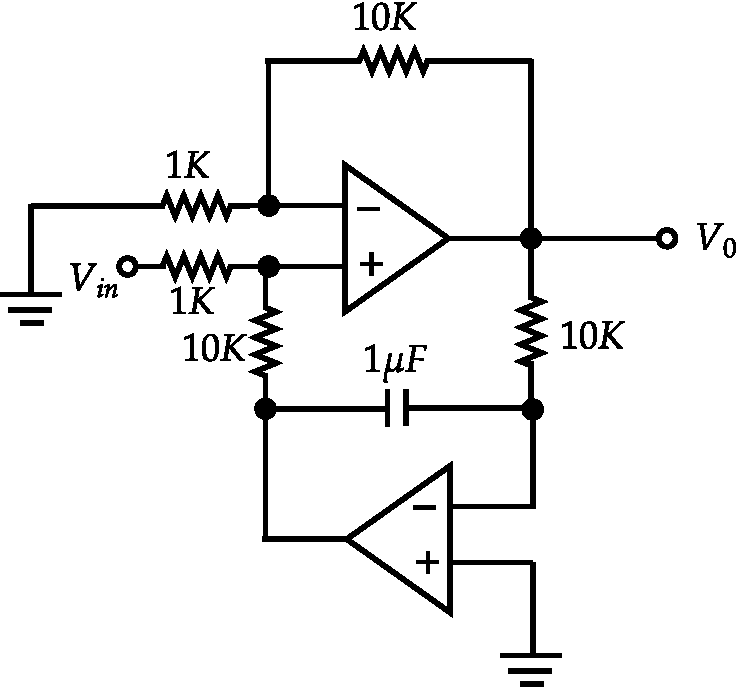
\includegraphics[height=6cm,width=6.5cm]{diagram-20211018(1)-crop}
	\end{figure}
	The circuit implements a
{	\exyear{NET/JRF(JUNE-2011)}}
\begin{tasks}(1)
\task[\textbf{A.}] High pass filter with cutoff frequency $16 \mathrm{~Hz}$
\task[\textbf{B.}] High pass filter with cutoff frequency $100 \mathrm{~Hz}$
\task[\textbf{C.}] Low pass filter with cutoff frequency $16 \mathrm{~Hz}$
\task[\textbf{D.}] Low pass filter with cutoff frequency $100 \mathrm{~Hz}$
\end{tasks}
\begin{answer}
\begin{align*}
\intertext{Since circuit has $R$ and $C$ combination, its a Low Pass filter and cutoff frequency}
&=\frac{1}{2 \pi R C} \approx 16 H z
\end{align*}
So the correct answer is \textbf{Option (C)}
\end{answer}
	\item The figure below shows a voltage regulator utilizing a Zener diode of breakdown voltage $5 \mathrm{~V}$ and a positive triangular wave input of amplitude $10 \mathrm{~V}$.\\
	\begin{figure}[H]
		\centering
		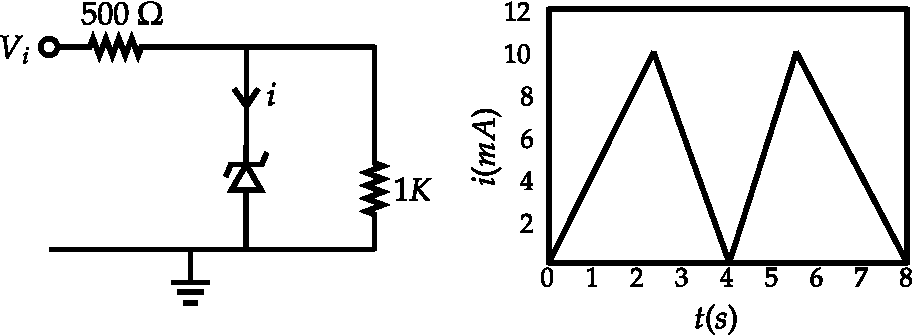
\includegraphics[height=3.5cm,width=8.5cm]{diagram-20211018(6)-crop}
	\end{figure}
	For $V_{i}>5 \mathrm{~V}$, the Zener regulates the output voltage by channeling the excess current through itself. Which of the following waveforms shows the current $i$ passing through the Zener diode?
{	\exyear{NET/JRF(DEC-2011)}}
\begin{tasks}(2)
\task[\textbf{A.}] \begin{figure}[H]
	\centering
	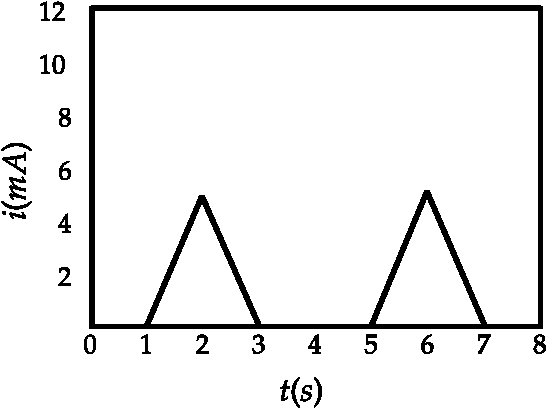
\includegraphics[height=3.3cm,width=5cm]{e-07a}
\end{figure}
\task[\textbf{B.}] \begin{figure}[H]
	\centering
	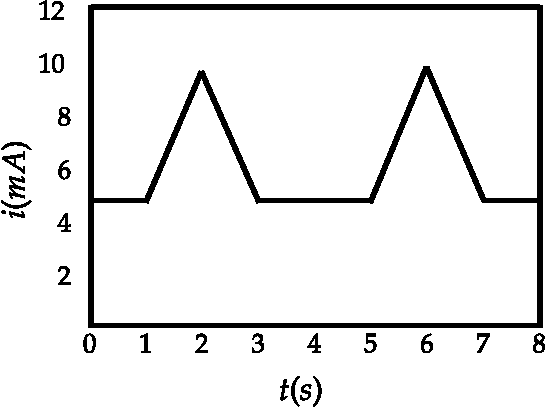
\includegraphics[height=3.3cm,width=5cm]{e-07b}
\end{figure}
\task[\textbf{C.}] \begin{figure}[H]
	\centering
	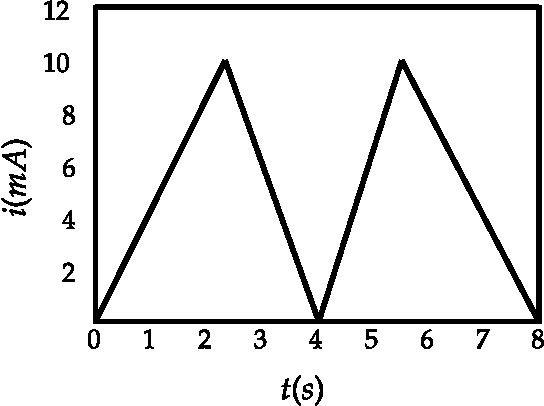
\includegraphics[height=3.3cm,width=5cm]{e-07c}
\end{figure}
\task[\textbf{D.}] \begin{figure}[H]
	\centering
	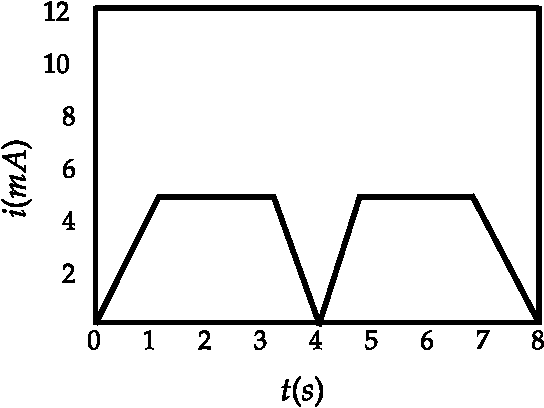
\includegraphics[height=3.3cm,width=5cm]{e-07d}
\end{figure}
\end{tasks}
\begin{answer}$\left. \right. $\\
When zener is OFF zener current is zero when zener is $\mathrm{ON}$ zener current will flow.\\
So the correct answer is \textbf{Option (A)}
\end{answer}
	\item In the op-amp circuit shown in the figure, $V_{i}$ is a sinusoidal input signal of frequency 10 $\mathrm{Hz}$ and $V_{0}$ is the output signal. The magnitude of the gain and the phase shift, respectively, close to the values
{	\exyear{NET/JRF(DEC-2012)}}
\begin{minipage}{0.45\textwidth}
\begin{tasks}(1)
	\task[\textbf{A.}] $5 \sqrt{2}$ and $\pi / 2$
	\task[\textbf{B.}] $5 \sqrt{2}$ and $-\pi / 2$
	\task[\textbf{C.}] 10 and zero
	\task[\textbf{D.}] 10 and $\pi$
\end{tasks}
\end{minipage}
\begin{minipage}{0.45\textwidth}
\begin{figure}[H]
	\centering
	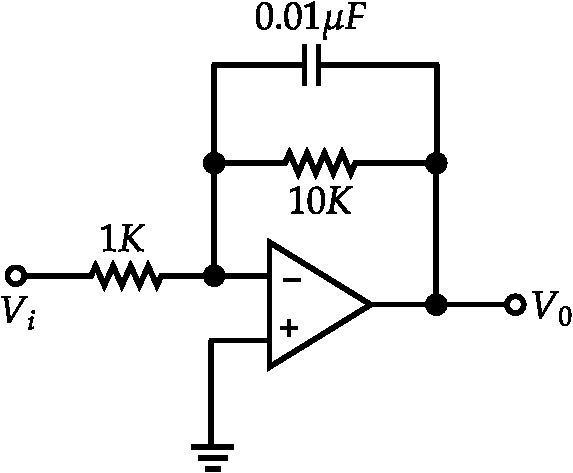
\includegraphics[height=4cm,width=5cm]{e-13}
\end{figure}
\end{minipage}
\begin{answer}
\begin{align*}
\frac{v_{0}}{v_{i n}}
&=-\frac{X_{C} R_{F}}{R_{1}\left(R_{1}+R_{F}\right)} \Rightarrow\left|\frac{v_{0}}{v_{i n}}\right| \approx 10
\end{align*}
So the correct answer is \textbf{Option (D)}
\end{answer}
	\item A diode $D$ as shown in the circuit has an $i-v$ relation that can be approximated by
	$$i_{D}=\left\{\begin{array}{ll}v_{D}^{2}+2 v_{D}, & \text { for } v_{D}>0 \\ 0, & \text { for } v_{D} \leq 0\end{array}\right.$$
	The value of $v_{D}$ in the circuit is
{	\exyear{NET/JRF(DEC-2012)}}
\begin{figure}[H]
\centering
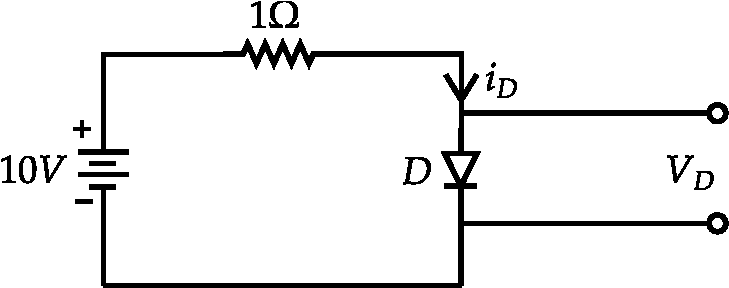
\includegraphics[height=3cm,width=6cm]{e-15}
\end{figure}
\begin{tasks}(4)
\task[\textbf{A.}] $(-1+\sqrt{11}) V$
\task[\textbf{B.}] $8 \mathrm{~V}$
\task[\textbf{C.}] $5 \mathrm{~V}$
\task[\textbf{D.}] $2 \mathrm{~V}$
\end{tasks}
\begin{answer}
\begin{align*}
-10+\left(v_{D}^{2}+2 v_{D}\right) \times 1+v_{D}&=0 \Rightarrow v_{D}=2 V
\end{align*}'
So the correct answer is \textbf{Option (D)}
\end{answer}
	\item A silicon transistor with built-in voltage $0.7 \mathrm{~V}$ is used in the circuit shown, with $V_{B B}=9.7 V, R_{B}=300 k \Omega, V_{C C}=12 V$ and $R_{C}=2 k \Omega$. Which of the following figures correctly represents the load line and quiescent $Q$ point?
{	\exyear{NET/JRF(JUNE-2013)}}
\begin{figure}[H]
\centering
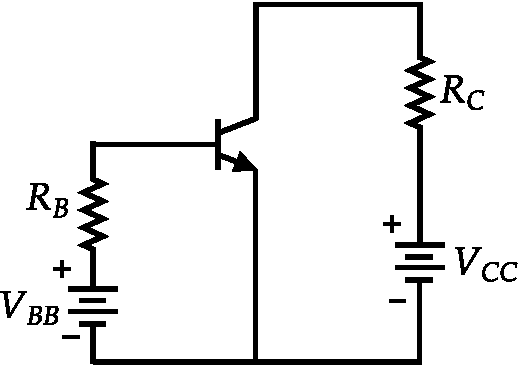
\includegraphics[height=3.5cm,width=5cm]{e-17}
\end{figure}
\begin{tasks}(2)
\task[\textbf{A.}] \begin{figure}[H]
	\centering
	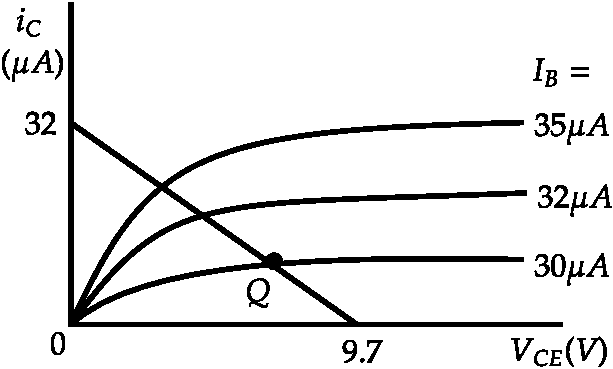
\includegraphics[height=3.3cm,width=5.5cm]{e-17a}
\end{figure}
\task[\textbf{B.}] \begin{figure}[H]
	\centering
	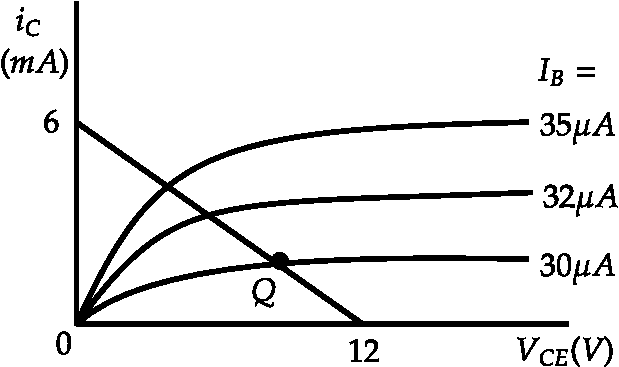
\includegraphics[height=3.3cm,width=5.5cm]{e-17b}
\end{figure}
\task[\textbf{C.}] \begin{figure}[H]
	\centering
	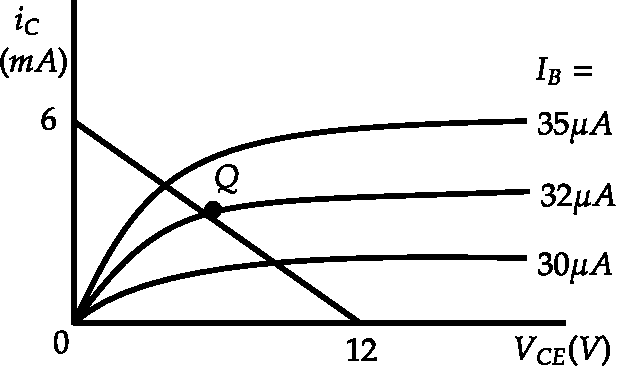
\includegraphics[height=3.3cm,width=5.5cm]{e-17c}
\end{figure}
\task[\textbf{D.}] \begin{figure}[H]
	\centering
	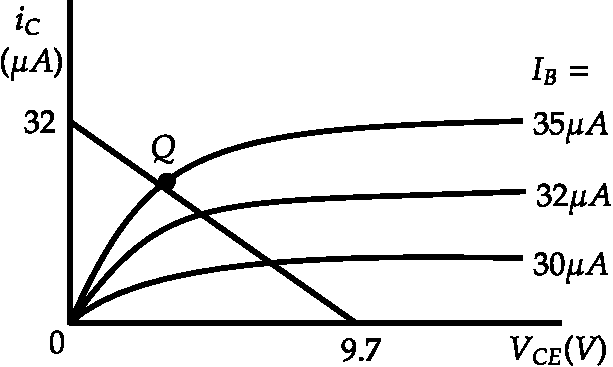
\includegraphics[height=3.3cm,width=5.5cm]{e-17d}
\end{figure}
\end{tasks}
\begin{answer}
\begin{align*}
I_{B}&=\frac{V_{B B}-V_{B E}}{R_{B}}=\frac{9.7-0.7}{300 \times 10^{3}}=30 \mu A\\\text{ and } I_{C, s a t}&=\frac{V_{C C}}{R_{C}}=\frac{12}{2 \times 10^{3}}=6 m A
\end{align*}
So the correct answer is \textbf{Option (B)}
\end{answer}
	\item Consider the op-amp circuit shown in the figure.
	If the input is a sinusoidal wave $V_{i}=5 \sin (1000 t)$, then the amplitude of the output $V_{0}$ is
{	\exyear{NET/JRF(DEC-2013)}}
\begin{figure}[H]
\centering
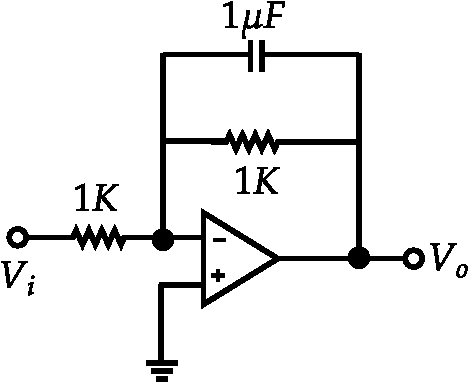
\includegraphics[height=3.5cm,width=4.5cm]{e-21}
\end{figure}
\begin{tasks}(4)
\task[\textbf{A.}] $\frac{5}{2}$
\task[\textbf{B.}]  5
\task[\textbf{C.}] $\frac{5 \sqrt{2}}{2}$
\task[\textbf{D.}] $5 \sqrt{2}$
\end{tasks}
\begin{answer}
\begin{align*}
\frac{v_{o}}{v_{\text {in }}}&=-\frac{X_{F}}{R_{1}}, X_{F}=\frac{R_{F} X_{C}}{R_{F}+X_{C}}=\frac{10^{3}}{(1+j)}\\\text{ where }R_{F}&=1 \times 10^{3} \Omega, X_{C}=\frac{1}{j \times 10^{3} \times 10^{-6}}\\
\left|\frac{v_{o}}{v_{i n}}\right|&=\frac{10^{3}}{\sqrt{2}} \times \frac{1}{10^{3}}=\frac{1}{\sqrt{2}} \Rightarrow v_{o}\\&=\frac{5}{\sqrt{2}} \sin \omega t=\frac{5 \sqrt{2}}{2} \sin \omega t
\end{align*}
So the correct answer is \textbf{Option (C)}
\end{answer}
	\item The $I-V$ characteristics of the diode in the circuit below is given by
	$$
	I=\left\{\begin{array}{rll}
	(V-0.7) / 500 & \text { for } & V \geq 0.7 \\
	0 & \text { for } & V<0.7
	\end{array}\right\}
	$$
	where $V$ is measured in volts and $I$ is measured in amperes.\\
	\begin{figure}[H]
		\centering
		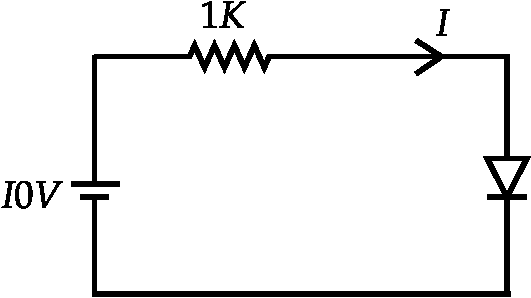
\includegraphics[height=2.5cm,width=4cm]{e-31}
	\end{figure}
	The current $I$ in the circuit is
{	\exyear{NET/JRF(DEC-2014)}}
\begin{tasks}(4)
\task[\textbf{A.}] $10.0 \mathrm{~mA}$
\task[\textbf{B.}] $9.3 \mathrm{~mA}$
\task[\textbf{C.}] $6.2 \mathrm{~mA}$
\task[\textbf{D.}] $6.7 \mathrm{~mA}$
\end{tasks}
\begin{answer}
\begin{align*}
\text{Applying K.V.L. }&-10+1000 \times I+V\\&=0 \Rightarrow-10+1000 \times(V-0.7) / 500+V=0\\
&\Rightarrow-10+2(V-0.7)+V\\&=0 \Rightarrow 3 V=11.4 \Rightarrow V=3.8\text{ Volts}\\
\text{Thus }I&=(V-0.7) / 500=(3.8-0.7) / 500\\&=3.1 / 500=6.2 \mathrm{~mA}
\end{align*}
So the correct answer is \textbf{Option (C)}
\end{answer}
	\item Analyse the ideal op-amp circuit in the figure. Which one of the following statements is true about the output voltage $V_{\text {out }}$, when terminal ' $C$ ' is connected to point ' $A$ ' and then to point ' $B$ '?
	{\exyear{JEST 2019}}
\begin{figure}[H]
\centering
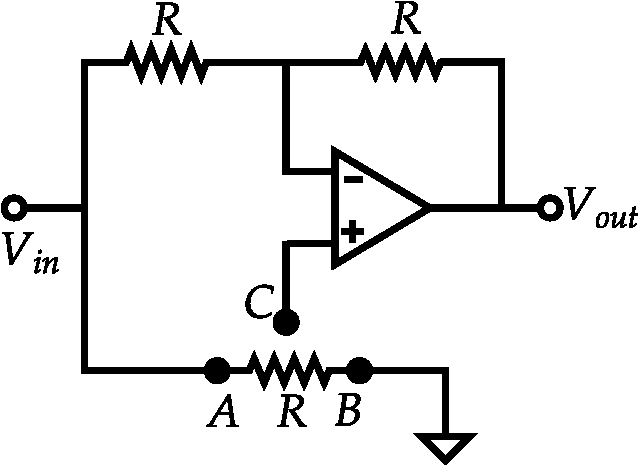
\includegraphics[height=4.5cm,width=6cm]{diagram-20210817(1)-crop}
\end{figure}
\begin{tasks}(1)
\task[\textbf{A.}] $V_{\text {out }}=V_{\text {in }}$ and $V_{\text {out }}=-V_{\text {in }}$ when ' $C$ ' is connected to ' $A$ ' and ' $B$ ', respectively
\task[\textbf{B.}] $V_{\text {out }}=-V_{\text {in }}$ and $V_{\text {out }}=V_{\text {in }}$ when ' $C$ ' is connected to ' $A$ ' and ' $B$ ', respectively
\task[\textbf{C.}] $V_{\text {out }}=-V_{\text {in }}$ when ' $C$ ' is connected to either ' $A$ ' or ' $B$ '
\task[\textbf{D.}]  $V_{\text {out }}=V_{\text {in }}$ when ' $C$ ' is connected to either ' $A$ ' or ' $B$ '
\end{tasks}
\begin{answer}
\begin{align*}
\intertext{	When terminal ' $C$ ' is connected to point ' $A$ '}
V_{\text {out }}&=\left(1+\frac{1}{1}\right) V_{\text {in }}-\frac{1}{1} V_{\text {in }}=V_{\text {in }}
\intertext{When terminal ' $C$ ' is connected to point ' $B$ '}
V_{\text {out }}&=-\frac{1}{1} V_{\text {in }}=-V_{\text {in }}
\end{align*}
So the correct answer is \textbf{Option (A)}
\end{answer}
	\item What is the voltage at the output of the following operational amplifier circuit. [See in the figure]?
{	\exyear{JEST 2015}}
\begin{figure}[H]
\centering
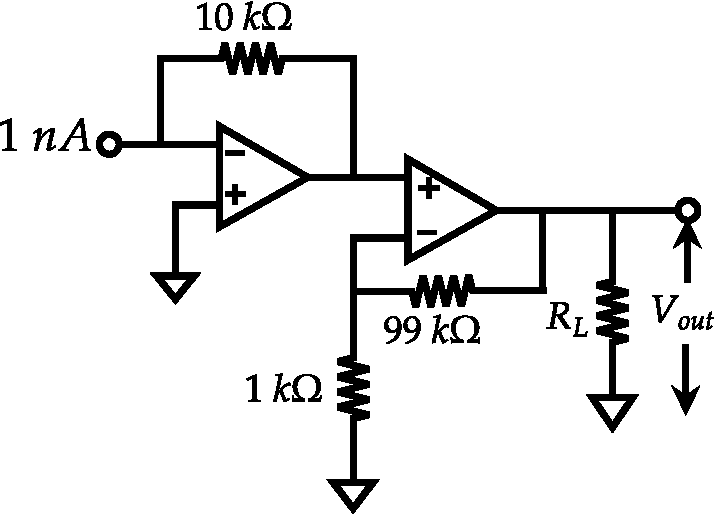
\includegraphics[height=5.5cm,width=7cm]{diagram-20210816(10)-crop}
\end{figure}
\begin{tasks}(4)
\task[\textbf{A.}] $1 \mathrm{~V}$
\task[\textbf{B.}] $1 \mathrm{mV}$
\task[\textbf{C.}] $1 \mu V$
\task[\textbf{D.}] $1 n V$
\end{tasks}
\begin{answer}
\begin{align*}
\text{Output of first Op-Amp }v_{01}&=-\left(10 \times 10^{3}\right)\left(1 \times 10^{-9}\right)\\&=-10^{-5} volt\\
\text{	Output of first Op-Amp }v_{\text {out }}&=\left(1+\frac{99}{1}\right) \times 10^{-5}\\&=10^{-3} volts =1 \mathrm{mV}
\end{align*}
So the correct answer is \textbf{Option (B)}
\end{answer}
	
	
	
	
	
	
	
	
	
	
	
	
	
	
	
	
	
	
	
	
\end{enumerate}